%%%%%%%%%%%%%%%%%%%%%%%%%%%%%%%%%%%%
% This is the template for submission to ISCA 2016
% The cls file is a modified from  'sig-alternate.cls'
%%%%%%%%%%%%%%%%%%%%%%%%%%%%%%%%%%%%

\documentclass{sig-alternate} 
\usepackage{mathptmx} % This is Times font

\newcommand{\ignore}[1]{}
\usepackage{fancyhdr}
\usepackage[normalem]{ulem}
\usepackage[hyphens]{url}
\usepackage{hyperref}

\usepackage{graphicx}
\usepackage{multirow}
\usepackage{breakurl}
\usepackage{tabularx}
\usepackage[nocompress]{cite}
\usepackage{subfig}
\usepackage{hyphenat}
\usepackage{xcolor}
\usepackage{dcolumn}
\newcolumntype{d}{D{.}{.}{2.1}}
\usepackage{flushend}
 \usepackage{pifont}
\newcommand*\mycirc[1]{{\large \ding{\numexpr201+#1\relax}}}

% required to break long URLS sanely
\PassOptionsToPackage{hyphens}{url} \usepackage{hyperref}
\expandafter\def\expandafter\UrlBreaks\expandafter{\UrlBreaks% save the current one 
\do\a\do\b\do\c\do\d\do\e\do\f\do\g\do\h\do\i\do\j% 
\do\k\do\l\do\m\do\n\do\o\do\p\do\q\do\r\do\s\do\t% 
\do\u\do\v\do\w\do\x\do\y\do\z\do\A\do\B\do\C\do\D% 
\do\E\do\F\do\G\do\H\do\I\do\J\do\K\do\L\do\M\do\N% 
\do\O\do\P\do\Q\do\R\do\S\do\T\do\U\do\V\do\W\do\X% 
\do\Y\do\Z\do\*\do\-\do\~\do\'\do\"\do\-}%

%%%%%%%%%%%---SETME-----%%%%%%%%%%%%%
\newcommand{\hpcasubmissionnumber}{18}
%%%%%%%%%%%%%%%%%%%%%%%%%%%%%%%%%%%%

\fancypagestyle{firstpage}{
  \fancyhf{}
\setlength{\headheight}{50pt}
\renewcommand{\headrulewidth}{0pt}
  \fancyhead[C]{\normalsize{ISCA 2016 Submission
      \textbf{\#\hpcasubmissionnumber} \\ Confidential Draft: DO NOT DISTRIBUTE}} 
  \pagenumbering{arabic}
}  

%%%%%%%%%%%---SETME-----%%%%%%%%%%%%%
\title{Thermostat} 
%\title{Managing Huge Pages In Two-Tiered Main Memory} 
\author{}
%\author{Neha Agarwal, Thomas F. Wenisch\\University of Michigan}
%%%%%%%%%%%%%%%%%%%%%%%%%%%%%%%%%%%%

\begin{document}
\maketitle
\thispagestyle{firstpage}
\pagestyle{plain}

\begin{abstract}
The advent of denser/cheaper memory technologies has renewed interest in
two-tiered main memory schemes, where cold data are shifted to slow memory to
enable greater capacity or reduce cost.  Past research on two-tiered main memory
has assumed a 4KB page size.  However, our recent work demonstrates that 2MB
(transparent) huge pages are performance critical in Cloud applications.  We
propose to develop a transparent huge-page-aware two-tiered memory solution,
targeting virtualized cloud applications, which integrates support for dynamic
page migration and transparent huge pages, achieving both the capacity/cost
advantages of two-tiered memory and performance advantages of huge pages. Hot
regions within otherwise cold huge pages present a central challenge to our
objective. We propose translation facades, a 4KB translation that remaps a
portion of a 2MB mapping with an alternate physical address or permissions, to
facilitate remapping hot portions of cold huge pages.
\end{abstract}

%\vspace{-0.05in}
\section{Introduction}
%\vspace{-0.05in}
%GPUs have enabled parallel processing for not just graphics applications but
%for a wide range of HPC installations and data-centers like Amazon's elastic
%compute cloud (EC2).  With this massively parallel processing often comes an
%insatiable demand for main memory bandwidth as GPUs churn through data at an
%ever increasing rate.  To meet this bandwidth demand, many GPUs have been
%designed with attached high-bandwidth GDDR memory rather than standard DDR
%memory used by CPUs.  As a result, many GPUs today have GDDR bandwidth that is
%2-5$\times$ higher than the memory bandwidth available to the CPU in the
%system.  To make best use of the bandwidth available to GPU programs
%programmers manually copy the data over the relatively slow PCIe bus to the GPU
%memory, and -- only then -- launch their GPU kernels.  This up-front data
%allocation and transfer has been necessary since transferring data over the
%PCIe bus is a high overhead operation, and a bulk transfer of data amortizes
%this overhead. This data manipulation overhead also results in significant
%porting challenges when retargeting existing applications to GPUs, particularly
%for high-level languages that make use of libraries and dynamic memory
%allocation during application execution.
%
%\begin{figure}[t]
%    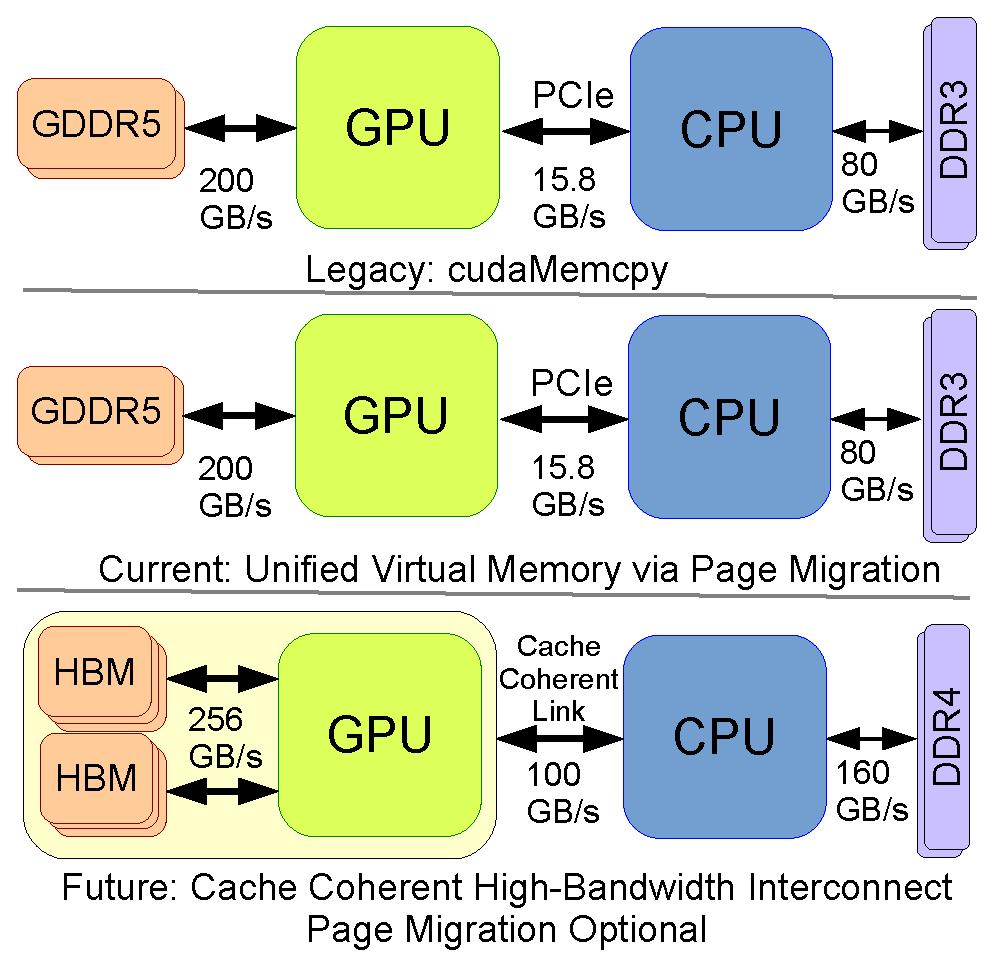
\includegraphics[width=\columnwidth]{hpca2015/figures/architecture.eps}
%    \caption{System architectures for legacy, current, and future mixed GPU-CPU systems.}
%    \label{fig:arch}
%\end{figure}
%
%Recognizing the obstacle this programming model poses to the wider adoption of
%GPUs in more parallel applications, programming systems like NVIDIA's CUDA,
%OpenCL, and OpenACC are evolving. Concurrently, GPU-CPU architectures are
%evolving to have unified globally addressable memory systems in which both the
%GPU and CPU can access any portion of memory at any time, regardless of its
%physical location.  Today this unified view of memory is layered on top of
%legacy hardware designs by implementing software-based runtimes that
%dynamically copy data on demand between the GPU and CPU~\cite{cuda}. As
%depicted in Figure~\ref{fig:arch}, over the next several years it is expected
%that GPU and CPU systems will move away from the PCIe interface to a fully
%cache coherent (CC) interface ~\cite{AMDHSA}. These systems will provide high
%bandwidth and low latency between the non-uniform memory access (NUMA) pools
%attached to discrete processors by layering coherence protocols on top of
%physical link technologies such as NVLink~\cite{NVLINK},
%Hypertransport~\cite{AMDHT}, or QPI~\cite{INTELQPI}.   CC-NUMA access to host
%memory from the GPU makes the software page migration used today an optional
%feature thanks to the improved bandwidth, latency, and access granularity that
%cache coherence can provides.
%
GPUs are throughput oriented processors that spawn thousands of threads
concurrently, demanding high memory bandwidth. To maximize the bandwidth
utilization programmers copy over the data to high bandwidth memory like GDDR5
before launching GPU kernels to amortize the overhead of accessing memory over
microsecond link latencies like PCIe. Hence, it is the responsibility of the
programmer to identify data that will be accessed by the GPU and copy it over to
the GPU-attached high bandwidth memory. NVIDIA's unified virtual
memory~\cite{UVM} has relaxed this constraint to enhance GPU programmability by
providing a software mechanism that performs on demand {\tt memcpy} of the data
as GPU accesses it. However, on demand data copying hurts GPU throughput. In
this chapter we discuss techniques of performing programmer agnostic dynamic
memory migration of performance critical data across CC-NUMA CPU-GPU system
connected by a next generation interconnect technology to maximize bandwidth
utilization, while not demanding the programmer to perform explicitly {\tt
memcpy(s)}.  We specifically examine how to best balance accesses through
cache-coherence and page migration.

%The contributions of this work are the following:

%While interconnect advancements improve GPU-CPU connectivity, no reduction is
%expected in the memory bandwidth differential between CPU and GPU-attached
%memory.  On-package memories such as High Bandwidth Memory (HBM) or Wide-IO2
%(WIO2) may in fact increase this differential as GPU bandwidth requirement
%continues to grow, feeding the ever increasing number of parallel cores
%available on GPUs used by both graphics and compute workloads. On the other
%hand, architects will likely continue to balance latency, power, and cost
%constraints against raw bandwidth improvement for CPU attached memory, where
%bandwidth and application performance are less strongly correlated. With
%application data residing primarily in CPU memory on application start-up, the
%GPU can access this memory either via hardware cache-coherence (which improves
%memory system transparency to the programmer) or by migrating a memory page into
%GPU physical memory (facilitating greater peak bandwidth for future requests).
%In this work we specifically examine how to best balance accesses through
%cache-coherence and page migration for a hypothetical CC-NUMA GPU-CPU system
%connected by a next generation interconnect technology.  The contributions of
%this work are the following:

%\begin{enumerate}
%\item
%1) Counter-based metrics to determine when to migrate pages from the CPU to GPU 
%are insufficient for finding an optimal migration policy to exploit GPU memory bandwidth. 
%In streaming workloads, where each page
%may be accessed only a few times, waiting for $N$ accesses to occur before
%migrating a page will actually limit the number of accesses that occur after
%migration, reducing the efficacy of the page migration operation.

%\item
%2) TLB shootdown and refill overhead can significantly degrade the
%performance of any page migration policy for GPUs\@. We show that combining reactive
%migration with virtual address locality information to aggressively prefetch pages
%can mitigate much of this overhead, resulting in increased GPU throughput.

%\item
%3) The legacy intuition to migrate all data to the GPU local memory in an attempt to maximize bandwidth fails to leverage
%the bandwidth available via the new CC-NUMA interface.  A page migration policy which 
%is aware of this differential and balances migration with CC-NUMA link
%utilization will outperform either GPU or GPU memory being used in isolation.

%\item 
%4) We present a software based memory placement system that, on average, outperforms CC-NUMA based
%accesses by 1.95$\times$, performs 6\% better than the legacy CPU to GPU {\tt
%memcpy} approach by 
%intelligently using both CPU and GPU memory bandwidth, and comes within 28\% of oracular page placement,
%all while maintaining the relaxed memory semantics of modern GPUs.
%\end{enumerate}

\vspace{-0.05in}
\section{Motivation and Background}
\label{background}
\vspace{-0.05in}

\begin{figure}[t]
        \includegraphics[width=\columnwidth]{hpca2015/figures/motivation.png}
    \caption{GPU performance sensitivity to memory subsystem performance where GDDR provides 
    200GB/s, DDR provides 80GB/s, and {\tt memcpy} bandwidth is 80GB/s.}
    \label{fig:motivation}
\end{figure}

A by-product of the GPU's many-threaded design is that
it is able to maintain a large number of in-flight memory requests and execution throughput
is correlated to memory bandwidth rather than latency, as compared to CPU designs.  As a result,
GPUs have chosen to integrate high bandwidth off-package memory like GDDR rather than accessing
the CPU's DDR directly or integrating DDR locally on the GPU board.  This choice is motivated
by our observation that the performance of some GPU compute workloads would degrade by as much as 
66\% if the traditional GDDR memory on a GPU were replaced with standard DDR memory, as seen in 
Figure~\ref{fig:motivation}.

In current CPU/GPU designs, GPU and CPU memory systems are private and require
explicit copying to the GPU before the application can execute.   Figure~\ref{fig:motivation}
shows the effect of this copy overhead on application performance by comparing GDDR to GDDR+{\tt memcpy}
performance which includes the cost of the programmer manually copying data from the DDR to the GDDR
before launching the GPU kernels.  While this copy overhead varies from application to application,
it can be a non-trivial performance overhead for short-running GPU applications and can even negate the 
effectiveness of using the high bandwidth GDDR on-board the GPU in a limited number of cases.

While it is technically possible for the GPU to access CPU memory directly over PCIe today, the long
latency (microseconds) of the access makes this a rarely used memory operation. 
Programming system
advancements enabling a uniform global address space, like those introduced in
CUDA 6.0~\cite{cuda}, relax the
requirement forcing programmers to allocate and explicitly copy memory to the GPU up-front, but
do nothing to improve the overhead of this data transfer. Further, by copying pages from the CPU to the GPU 
piece-meal on demand, these new runtimes often introduce additional overhead compared to
performing a highly optimized bulk transfer of all the data that the GPU will need during execution.
The next step in the evolution of GPUs, given the unified addressing, is
to optimize the performance of this new programming model. 

\subsection {Cache Coherent GPUs}

The key advancement expected to enable
performance is the introduction of CC-NUMA GPU and CPU systems.  Using cache coherence layered upon NVLink, HT, or QPI, GPUs will
likely be able to access CPU memory in hundreds of nanoseconds at bandwidths up to 128GB/s by bringing
cache lines directly into GPU caches. Figure~\ref{fig:motivation} shows the upper bound (labeled ORACLE) on performance
that could be achieved if both the system DDR memory and GPU GDDR memory were used concurrently, assuming data had 
been optimally placed in both technologies.  In this work, we define oracle placement to be \emph{a priori} page placement
in the GPU memory (thus requiring no migration), of the minimum number of pages, when sorted from hottest to coldest, 
such that the GDDR bandwidth is fully subscribed during application execution.

Because initial CPU/GPU CC-NUMA systems are likely to use a form of IOMMU address translation services 
for walking the OS page tables within the GPU,  it is unlikely that GPUs will be able to directly
allocate and map their own physical memory without a call back to the CPU and operating system.
In this work, we make a baseline assumption that all physically allocated pages are initially allocated
in the CPU memory and only the operating system or GPU runtime system executing on the host can initiate
page migrations to the GPU\@.  In such a system, two clear performance goals become evident.
The first is to design a memory policy that balances CC-NUMA access and page migration to simply achieve the 
performance of the legacy bulk copy interface without the programming limitations.  The second, more ambitious, goal
is to exceed this performance and approach the oracular performance by using these memory zones concurrently, enabling 
a peak memory bandwidth that is the sum of the two zones.

Achieving either of these goals requires
migrating enough data to the GPU to exploit its high memory bandwidth while avoiding migrating pages
that may never be accessed again.  Every page migration increases the total bandwidth requirement of the
application and over-migration potentially reduces application performance if sufficient bandwidth headroom in both the DDR and GDDR is not available.
Thus, the runtime system must be selective about which pages to migrate.  The runtime system also must be cognizant
that performing TLB invalidations (an integral part of page migration) on a GPU does not just halt a single
processor, but thousands of compute pipelines that may be accessing these pages through a large shared TLB structure.
This shared TLB structure makes page migrations between a CPU and GPU potentially much more costly (in terms of the opportunity cost of lost execution throughput) than in CPU-only systems.

In addition to managing the memory bandwidth overhead
of page migration and execution stalls due to TLB shootdowns, the relative bandwidth utilization of both the CPU and GPU memory 
must be taken into account when making page migration decisions.  When trying to balance memory bandwidth between two distinct memory
zones, it is possible to over- or under-subscribe either memory zone. Migrating pages too slowly to the GPU
memory will leave its local memory sitting idle, wasting precious bandwidth.  Conversely, migrating pages
to the GPU too aggressively may result in under-utilization of the CPU memory while paying the maximum cost in terms
of migration overheads. A comprehensive CPU-GPU memory management solution will attempt to balance all of 
these effects to maximize memory system and GPU throughput in future mobile, graphics, HPC, and datacenter
installations.

\subsection{Related Work}
\label{related_work}
\vspace{-0.05in}

Using mixed DRAM technologies or DRAM in conjunction with non-volatile memories
to improve power consumption on CPUs has been explored by several groups
~\cite{Kultursay2013,Phadke11mlpaware2011,Mogul2009,Bheda2011,Ramos2011}.
The majority of this work attempts to overcome the performance reductions introduced
by non-DDR technologies to improve capacity, power consumption, or both.
In CC-NUMA systems, there has been a long tradition of examining where to place
memory pages and processes for optimal performance, typically focusing on reducing
memory latency~\cite{Wilson2001,Bolosky1989,Brecht1993,LaRowe1992,Verghese1996,Iyer1998}.
Whereas CPUs are highly sensitive to memory latency, GPUs can cover a much larger latency
through the use of multi-threading.  More recent work on page placement and 
migration~\cite{AUTONUMA,Dashti2013,Tam2007,Zhuravlev2010,Knauerhase2008,Blagodurov2011,awasthinellans10}
has considered data sharing characteristics, interconnect utilization, and memory controller
queuing delays in the context of CPU page placement. However, the primary improvements in many of these works,
reducing average memory latency, will not directly apply in a GPU optimized memory system.

Several recent papers have explored hybrid DRAM-NVM GPU attached memory subsystems~\cite{zhao2013,Wang2013}.
Both of these works consider a traditional GPU model where the availability of low latency, high bandwidth access to CPU-attached 
memory is not considered, nor are the overheads of moving data from the host CPU onto the GPU considered.
Several papers propose using a limited capacity, high bandwidth memory as a
cache for a larger slower memory~\cite{jiang2011,Meza2012}, but such designs incur a high engineering
overhead and would require close collaboration between GPU and CPU vendors that often do not
have identically aligned visions of future computing systems.

When designing page migration policies, the impact of TLB shootdown overheads and page table updates is a constant
issue.  Though most details about GPU TLBs are not public,
several recent papers have provided proposals about how to efficiently implement general purpose TLBs
that are, or could be, optimized for a GPU's needs~\cite{Pichai2014,Villavieja2011,Power2014}. Others
have recently looked at improving TLB reach by exploiting locality within the virtual to physical
memory remapping, or avoiding this layer completely~\cite{swansonstoller98,Pham2014,Basu2013}.  
Finally, Gerofi et al.~\cite{Gerofi2014} recently examined TLB performance of the Xeon Phi
for applications with large footprints, while McCurdy et al.~\cite{McCurdy2008} investigated the
effect of superpages and TLB coverage for HPC applications in the context of CPUs.

\section{Proposal: Thermostat}
\label{proposal}

End-to-end Linux Prototype with minimal hardware changes to employ
slower but cheaper memory in data-centers.

\subsection{Identifying HotSpots in Cold Hugepages}

\begin{figure}[t]
\centering
\includegraphics[width=1.0\columnwidth]{thermostat/figures/sampling.png}
\caption{Sampling to identify HotSpot pages in otherwise cold page}
\vspace{-0.175in}
\label{fig:sampling}
\end{figure}
To solve this situation, we propose to build a dynamic controller (which we call
Thermostat) that can decide when to {\it break} a huge page into several regular
pages, and place some of those smaller pages which are deemed to be cold in
slower but cheaper memory. We will implement Thermostat as a part of custom
Linux prototype. The following design issues arise when creating this Thermostat
controller.

First, the Thermostat controller has to distinguish between ``hotSpot'' hot pages -- ones
with only a few hot data blocks, and ``uniform'' hot pages -- ones where a
significant fraction of the data blocks in that page are hot.  We propose to
build such a classification mechanism that is at once a)
application-transparent, i.e., no source code change in the application should
be necessary, b) low-overhead, so as to not degrade the performance benefits of
using THP, and, c) high-accuracy, i.e., most of the classified ``hotSpot'' pages
are indeed hotspots (low false positives) and most of the pages classified
``uniform'' are {\it} not in fact hotspots (low false negatives).

We observe that there are hot 4KB pages present within 2MB huge pages.
Figure~\ref{fig:motivation-thermostat}
shows that applications on average have $\approx$ 50\% of cold data. As we change page size
form 4KB to 2MB fraction of cold data reduced by $\approx$ 50\%. Page granularity based
OS mechanisms cannot reveal the hot portions within huge pages. Hence, we
propose a sampling based page temperature measurement mechanism that classifies
pages by their access rate.

\subsection{Translation Facades}

%\begin{figure}[t]
%\centering
%\includegraphics[width=1.0\columnwidth]{thermostat/figures/sampling.png}
%\caption{TLB and PTE changes}
%\vspace{-0.175in}
%\label{fig:motivation}
%\end{figure}
%
Second, the Thermostat controller needs an effective mechanism for chunking up a DRAM
huge page into several small pages, and also for compacting several small hot
pages into a single DRAM huge page. Chunking up a huge page is relatively simple
-- one need only allocate several page table entries (PTEs) corresponding to the
chunked up page. Doing the inverse, that is compacting several small pages from
the slow-mem and DRAM into a single DRAM huge page has more challenges. First,
due to memory fragmentation, it may not be possible to find a suitable space to
put the newly created huge page. Second, reading several small pages from
slow-mem, and creating a huge page out of them can be a potentially very long
latency operation, which can then affect application throughput as well as tail
latency. We plan to study the design trade-off space of when to perform
these operations and incorporate the obtained insights into building the Thermostat
controller.

\section{Methodology}
\label{section:methodology}

\subsection{System Configuration}
We study Thermostat on  a 36-core (72 hardware thread) dual-socket
x86 server, Intel Xeon E5-2699 v3, with 512 GB RAM running Linux 4.5.
Each socket has 45MB LLC. There is a 64-entry TLB per core and a shared 1024
entry L2 TLB. Several of our benchmark applications perform frequent I/O and are
highly sensitive to OS page cache performance.
To improve the page cache, we install {\tt hugetmpfs}, a mechanism that
enables use of huge pages for the {\tt tmpfs}~\cite{hughd-hugetmpfs} filesystem. 
We place all files accessed by the benchmarks in {\tt tmpfs}. In the future, we expect
that Linux may natively support huge pages in the page cache for other file
systems.

We run the benchmarks inside virtual machines using the Kernel-based Virtual
Machine (KVM) virtualization platform.  Client threads, which generate traffic to the
servers, are run outside the virtual machine, on the host OS. We run the client threads 
and server VM on the same system and use a bridge network with virtio between host 
and guest so that network performance is not a bottleneck.
We isolate the CPU and
memory of the guest VM and client threads on separate sockets using 
Linux's control group mechanism~\cite{cgroups} to avoid performance interference.  
The benchmark VM is allocated 8 CPU cores, a typical medium-sized cloud 
instance.
We set the Linux frequency governor to ``performance'' to
disable dynamic CPU frequency changes during application runs. 

\subsection{Emulating slow memory: BadgerTrap}
\label{slow-memory}
Dual-technology main memory, in particular Intel/Micron's 3D XPoint memory, 
is not yet available.  
Hence, we use a software technique to emulate slow memory while placing all
data in conventional DRAM.

Each cache miss to slow memory should incur an access latency that is a multiple 
of the DRAM latency (e.g., 400ns slow memory~\cite{ref:Dulloor:datatiering} vs. 
50ns DRAM latency).
There is no easy mechanism to trap to software on all cache misses. Instead,
we introduce extra latency by inducing page faults upon translation misses (TLB misses) 
to cold pages by using BadgerTrap~\cite{ref:badgertrap}. 
%This mechanism is similar to 
%how Thermostat measures page access frequency.

The software fault mechanism is an approximation of an actual slow memory device.
The BadgerTrap fault latency (about 1us in our kernel) is higher than some authors
predict the 3D XPoint memory read latency will be~\cite{ref:Dulloor:datatiering}.  Furthermore, the poisoned PTE
will induce a fault even if the accessed memory location is present in the hardware 
caches. In these two respects, our approach over-estimates the penalty of slow 
memory accesses.  However, once BadgerTrap installs a (temporary) translation, 
further accesses to other cache blocks on the same slow-memory page will not 
induce additional faults, potentially under-estimating impact. Our testing with micro benchmarks
indicates our approach yields an average access latency to slow memory in the 
desired range, in part, because slow-page accesses are sufficiently infrequent that
they nearly always result in both cache and TLB misses anyway, as we discuss in
Section~\ref{section:access-counting}.
%On balance, we expect the differences between
%TLB and cache misses to have little impact because, by design, Thermostat places
%only rarely accessed pages in cold memory.

%We validate that BadgerTrap provides a reasonable approximation of slow memory
%by measuring the TLB and cache miss rates for our benchmark suite using hardware
%performance counters.  The TLB miss rate induced by BadgerTrap is typically higher 
%(but always within a factor of two) than the last-level cache miss rate measured 
%without BadgerTrap, indicating that our performance estimates are conservative.
%\fixme{Neha: Verify this number for all the new benchmarks.}

One important detail of our test setup is that we must install BadgerTrap (for the purpose 
of emulating slow memory latency) within
the guest VM rather than the host OS.  Thermostat communicates with the guest-OS 
BadgerTrap instance to emulate migration to slow memory.  We must install
BadgerTrap within the guest because, otherwise, each BadgerTrap fault would 
result in a {\tt vmexit}.  In addition to drastically higher fault latency, {\tt vmexit} operations
have the side-effect of changing the Virtual Processor ID (VPID) to 0. Since KVM
uses VPIDs to tag TLB entries of its guests, installing a TLB entry with the
correct VPID would entail complexity and incur even higher emulation latency.
% than
%involve a significantly complex operation of re-entering the
%VM, performing a single memory operation and jumping back, which would incur
%even more emulation latency.
Since BadgerTrap on the guest entails a latency of
$\approx$ 1$\mu$s, which is already higher than projected slow-memory latencies~\cite{ref:Dulloor:datatiering},
we did not want to incur additional slowdown by emulating slow memory in the
host OS.


%To ensure that this approach is
%reasonable, we obtained the TLB and cache miss rates for the applications under
%study by {\tt perf}. We observed that in Cassandra and MySQL-TPCC the TLB miss
%rate (resulting into page walks)
%was 2$\times$ higher than the last level cache miss rate, meaning that we will only be
%overestimating the performance impact. In Redis, however, the TLB miss rate is
%2$\times$ lower than the cache miss rate. 

%{\textbf{Why not Badgertrap on the host?}


\subsection{Benchmarks}
\label{benchmarks}
We evaluate Thermostat with applications from Google's Perfkit Benchmarker and
the Cloudsuite benchmarks~\cite{perfkitbenchmarker, cloudsuite}. These
applications are representative server workloads that have large memory
footprints and are commonly run in virtualized cloud environments.  We do not
evaluate Thermostat for general-purpose GPU applications since non-volatile memory
technologies are expected to have much lower bandwidth than high-bandwidth
graphics memories -- even lower than DDR memory technologies -- thus are not a
suitable match to memory bandwidth-sensitive platforms like GPUs.

{\bf TPCC on MySQL:} TPCC is a widely-used database benchmark, which aims to measure
the transaction processing throughput of a relational database~\cite{tpcc}. We 
execute TPCC on top of MySQL, one of the most popular open-source database 
engines, which is often deployed in the cloud.  We use the open-source
TPCC implementation from OLTP-Bench~\cite{oltpbench} (available at
\url{https://github.com/oltpbenchmark/oltpbench}). We use a scale factor of
320, and run the benchmark for 600 seconds after warming up for 600 seconds.
MySQL makes frequent I/O requests and hence benefits markedly from our use
of {\tt hugetmpfs} to enable huge pages for the OS page cache.
%We observe 380
%transactions/sec throughput for our baseline system with all pages in DRAM as
%huge pages.

{\bf NoSQL databases:} Aerospike, Cassandra, and Redis are popular NoSQL
databases~\cite{aerospike, cassandra, redis}.
Cassandra is a wide-column database designed to offer a variable number of fields
(or columns) per key, while Redis and Aerospike are simpler key-value databases 
that have higher peak throughput. Redis is single-threaded whereas Aerospike is
multi-threaded.
Cassandra performs frequent file I/O as it periodically compacts its SSTable
data structure on disk~\cite{ref:sstable}. So, Cassandra also benefits substantially
from {\tt hugetmpfs}. Redis performs no file I/O after loading its dataset into memory.

We tune Aerospike, Cassandra, and Redis based on the settings provided by
Google's Perfkit Benchkmarker for measuring cloud
offerings~\cite{perfkitbenchmarker}.  We use the YCSB traffic generator to drive
the NoSQL databases~\cite{ycsb}. For Aerospike we use 200M operations
and for Cassandra we use 50M operations on 5M keys with 20 fields each with a
Zipfian distribution.
For both of these application, we evaluate two workload mixes: a read-heavy load
with 95:5 read/write ratio and a write-heavy load with 5:95 read/write ratio. For Redis, we
access keys with a hotspot distribution, wherein 0.01\% of the keys account for
90\% of the traffic. We vary value sizes according to the
distribution reported in~\cite{facebook-key-value}. We observe 176K
and 215K operations/sec for read-heavy and write-heavy workloads for Aerospike,
and 21K and 45K operations/sec for read-heavy and write-heavy workloads for
Cassandra. For Redis we observe 188K
operations/sec for our baseline system with all pages in
DRAM as huge pages.

{\bf In-memory analytics:} We evaluate Thermostat on in-memory analytics
benchmarks from Cloudsuite~\cite{cloudsuite}. In-memory analytics runs a
collaborative filtering algorithm on a dataset of user-movie ratings.  It uses
the Apache Spark framework to perform data analytics. We set both executor and driver
memory to be 6GB to execute the benchmark entirely in memory. We run the benchmark to
completion, which takes 317 seconds for our baseline system with all pages in
DRAM as huge pages.

{\bf Web search:} Cloudsuite's web search uses the Apache Solr search engine
framework. We run client threads on host and index nodes within the virtual
machine. We set steady state time to be 300 seconds and keep default values for all
the other parameters on the client machine. As specified by the benchmark,
target response time requires 99\% of the requests to be serviced in 200ms. For
our baseline system with all pages in DRAM as huge pages, we observe 50
operations/sec with $\approx$ 85ms 99th percentile latency.
%{\bf Tomcat:} Tomcat is a popular web server frontend. We use the {\tt wrk}
%(available at \url{https://github.com/wg/wrk}) tool to generate XXX requests to
%the webpage \texttt{XXX.XXX} using XXX parallel clients. Our installation runs
%at the peak throughput at this load. 

\subsection{Runtime overhead of Thermostat Sampling}
We measure the runtime overhead of Thermostat to ensure that application 
throughput is not degraded by Thermostat's page sampling mechanism.
For sampling periods of 10s or higher, we observe negligible CPU activity
from Thermostat and no measurable application slowdown ($<$ 1\%).


\begin{table}[t]
\begin{center}
\begin{tabular}{|l|l|l|}
\hline
& Resident Set Size& File-mapped\\
\hline
Aerospike & 12.3GB & 5MB\\
\hline
Cassandra & 8GB & 4GB\\
\hline
MySQL-TPCC & 6GB & 3.5GB\\
\hline
Redis & 17.2GB & 1MB\\
\hline
%Graph-analytics & 16.6GB & 1MB\\
%\hline
In-memory-analytics & 6.2GB & 1MB\\
\hline
Web-search & 2.28GB & 86MB\\
\hline
\end{tabular}
%\vspace{0.05in}
\caption{Application memory footprints: resident set size and file-mapped pages.}
\label{tab:memory-footprint}
\end{center}
\end{table}

\section{Results}
\label{results}
We evaluate the performance of selective GPU caching through iterative addition of our three proposed microarchitectural
enhancements on top of naive selective caching. We then add promiscuous read-only caching and 
finally present a sensitivity study for scenarios where the workload footprint is too large for a 
performance-optimal page placement split across CPU and GPU memory.

\subsection{Microarchitectural Enhancements}
Figure~\ref{fig:uncachableperformance} shows the baseline performance of naive selective caching
compared to a hardware cache-coherent GPU.  Whereas performance remains as high as 95\% of the baseline 
for some applications,
the majority of applications suffer significant degradation, with applications like \texttt{btree}
and \texttt{comd} seeing nearly an order-of-magnitude slowdown.  The applications that are hurt most
by naive selective caching tend to be those that have a high L2 cache hit rate
in a hardware cache-coherent GPU
implementation like \texttt{comd} (Table~\ref{tab:gpuhitrate}) or those that are highly sensitive to L2 cache latency
like \texttt{btree} (Figure~\ref{fig:cache_bw_latency}).  Prohibiting all caching of CPU 
memory results in significant over-subscription of the CPU
memory system, which quickly becomes the bottleneck for application forward progress, resulting in
nearly a 50\% performance degradation across our workload suite.

\begin{figure}[t]
\includegraphics[width=1.0\columnwidth]{hpca2016/figures/unconstrainedperformance.png}
\caption{GPU performance under selective caching with uncoalesced requests, L1 coalesced requests,
L1+L2 coalesced requests.}
\label{fig:uncachableperformance}
\end{figure}

\subsubsection{Cacheless Request Coalescing}
\label{mshrresults}
Our first microarchitectural proposal is to implement cacheless request coalescing as described in Section~\ref{coalescing}.
With naive selective caching relying on only the lane-level request coalescer, performance of the system degrades 
to just 42\% of the hardware cache-coherent GPU, despite only 20\% of the application data residing in CPU physical memory.  
Introducing request coalescing improves performance to 74\% and 79\% of a
hardware cache-coherent GPU
when using L1 coalescing and L1+L2 coalescing, respectively.  This improvement comes from
a drastic reduction in the total number of requests issued across the CPU--GPU
interconnect and reducing pressure on the CPU memory. Surprisingly \texttt{srad\_v1} shows
a 5\% speedup over the hardware cache-coherent GPU when using L1+L2 request coalescing. \texttt{srad\_v1} has 
a large number of pages
that are written without first being read, thus the CPU DRAM system benefits from the elimination of reads that are caused
by the write-allocate policy in the baseline GPU's L2 cache.
Because the request coalescing hit rates, shown in
Table~\ref{tab:coalescing_opportunity}, lag behind the hardware cached hit rates,
selective caching still places a higher load on the interconnect and CPU memory
than a hardware cache-coherent GPU, which translates
into the 21\% performance reduction we observe when using selective caching with aggressive request coalescing.

\begin{figure}[t]
\includegraphics[width=1.0\columnwidth]{hpca2016/figures/unconstrainedperformanceMshrMCCache.png}
\caption{GPU performance with selective caching when combining request coalescing with on CPU-side
caching for GPU clients at 64KB--1MB cache capacities. (CC: Client-Cache)}
\label{fig:mccache}
\end{figure}

\subsubsection{CPU-side Client Cache}
\label{mccache}
Whereas request coalescing captures much of the spatial locality provided by GPU L1 caches, it cannot capture
any long distance temporal locality. Figure~\ref{fig:mccache} shows
the performance differential of adding our proposed CPU-side client cache to L1+L2 request coalescing within the selective
caching GPU. This GPU client cache not only reduces traffic to CPU DRAM from the GPU, but also improves latency for requests
that hit in the cache and provides additional bandwidth that the CPU--GPU interconnect may exploit.  We observe
that performance improvements scale with client cache size up to 512KB before returns diminish.  Combining
a 512KB, 8-way associative client cache with request coalescing improves
performance of our selective caching GPU to within 90\% of the performance of a
hardware cache-coherent GPU\@. Note that \texttt{btree} only benefits marginally from
this client cache because accessing the client cache still requires a round-trip interconnect
latency of 200ns (Section~\ref{methodology}). \texttt{btree} is highly sensitive to
average memory access latency (Figure~\ref{fig:cache_bw_latency}), which is not substantially improved by
placing the client cache on the CPU-die rather than the GPU-die.

The size of an on-die CPU client cache is likely out of the hands of GPU architects, and
for CPU architects allocating on-die resources for an external GPU client may seem an
unlikely design choice.  However, this client cache constitutes only a small fraction of the
total chip area of modern CPUs (0.7\% in 8-core Xeon E5~\cite{XeonLLC2013}) and is the size of just one additional private L2 cache
within the IBM Power 8 processor.  Much like processors have moved towards on-die integration of PCIe to provide improved performance
with external peripherals, we believe the performance improvements due to this cache are significant enough to warrant integration. 
For CPU design teams, integrating such a cache into an existing design is likely easier than achieving performance by extending
coherence protocols into externally developed GPUs. The GPU client cache also need not be specific to just GPU clients,
other accelerators such as FPGAs or spatial architectures~\cite{Putnam2014,Parashar2013} that will be integrated along-side a traditional
CPU architecture will also likely benefit from such a client cache.

\begin{figure}[t]
\includegraphics[width=1.0\columnwidth]{hpca2016/figures/linkimprovements.png}
\caption{GPU data transferred across CPU-GPU interconnect (shown left y-axis) and performance (shown right y-axis)
for 128B cache line-size link transfers and variable-size link transfers respectively.}
\label{fig:linkoptimization}
\end{figure}

\begin{figure}[t]
\includegraphics[width=1.0\columnwidth]{hpca2016/figures/readonlycaching.png}
\caption{GPU performance when using Selective caching (Request-Coalescing +
512kB-CC + Variable-Transfers) combined with read-only
based caching. geo-mean*: Geometric mean excluding \texttt{backprop, cns,
needle}, where read-only caching would be switched-off. (RO: Read-Only)}
\label{fig:readonlycaching}
\vspace{-0.1in}
\end{figure}

\subsubsection{Variable-size Link Transfers}
\label{linkoptimization}
Request coalescing combined with the CPU client cache effectively reduce the pressure on the CPU DRAM by limiting
the number of redundant requests that are made to CPU memory.  The CPU client cache exploits temporal locality
to offset data overfetch that occurs on the DRAM pins when transferring data at cache line granularity, but
does not address CPU--GPU interconnect transfer inefficiency.
To reduce this interconnect over-fetch, we propose variable-sized transfer units
(see Section~\ref{variablesizing}). The leftmost two bars for each benchmark in Figure~\ref{fig:linkoptimization} show the total traffic across the
CPU--GPU interconnect when using traditional fixed 128B cache line requests and
variable-sized transfers, compared to a hardware cache-coherent
GPU.  We see that despite request coalescing, our selective caching GPU transfers nearly 4 times the data
across the CPU--GPU interconnect than the hardware cache-coherent GPU.  Our variable-sized transfer
implementation reduces this overhead by nearly one third to just 2.6x more
interconnect traffic than the hardware cache-coherent GPU.

This reduction in interconnect bandwidth results in performance gains of just
3\% on average, despite some applications like {\tt comd} showing significant improvements. 
We observe that variable-sized transfers can significantly improve bandwidth utilization
on the CPU--GPU interconnect but most applications remain performance-limited by the CPU memory 
bandwidth, not the interconnect itself. When we increase interconnect bandwidth by 1.5x without enabling variable-sized
requests, we see an average performance improvement of only 1\% across our benchmark suite.
Variable-sized requests are not without value, however;
transferring less data will save power or allow this expensive off-chip interface to be clocked at a lower
frequency, but evaluating the effect of those improvements is beyond the scope of this work.

\subsection{Promiscuous GPU Caching}
\label{readonlyresults}
By augmenting selective caching with request coalescing, a GPU client cache, and variable-sized transfers,
we achieve performance within 93\% of a hardware cache-coherent GPU\@. 
As described in Section~\ref{readonly}, the GPU can be allowed to cache CPU memory that is contained
within pages that are marked as read-only by the operating system. The benefit of caching data
from such pages is offset by protection
faults and software recovery if pages promiscuously marked as read-only 
and cached by the GPU are later written.
Figure~\ref{fig:readonlycaching} (RO-ZeroCost) shows the upper bound on possible improvements from read-only 
caching for an idealized implementation that marks all pages as read-only and transitions them to
read-write (and thus uncacheable)
without incurring any cost when executing the required protection fault handling routine.  In a few cases, 
this idealized implementation can outperform 
the hardware cache-coherent GPU because of the elimination of write allocations in the GPU caches,
which tend to have little to no reuse.

We next measure the impact of protection fault cost, varying the unloaded fault latency from
20us to 40us (see Figure~\ref{fig:readonlycaching}) which is available on today's GPU implementations.
While a fault is outstanding, the faulting warp and any other warp that accesses
the same address are stalled; but, other warps may proceed, mitigating the impact of these faults on SM forward progress.  
The latency of faults can can be hidden if some warps executing on an SM are reading
this or other pages.  However, if all warps issue writes at
roughly the same time, the SM may stall due to a lack of schedulable warps or MSHR
capacity to track pending faults. When accounting for fault overheads, 
our selective caching GPU with promiscuous read-only caching achieves only 89\% of the performance of the 
hardware cache-coherent GPU.

When using a 20us fault latency, we see that 7 of 12 workloads 
exhibit improvement from read-only caching
and that \texttt{btree} sees a large 35\% performance gain from promiscuous read-only caching
as it benefits from improvements to average memory
access latency.
In contrast, three workloads, \texttt{backprop}, \texttt{cns}, and
\texttt{needle}, suffer considerable slowdowns due to exposed protection fault latency.
These workloads tend to issue many concurrent writes, exhausting the GPUs
ability to overlap execution with the faults.  For such workloads, we advocate
disabling promiscuous read-only caching in software (e.g., via a mechanism that tracks
the rate of protection faults, disabling promiscuous read-only caching when the rate
exceeds a threshold).

In summary, the effectiveness of promiscuous read-only caching depends heavily on
the latency of protection faults and the GPU microarchitecture's ability to overlap the
execution of non-faulting warps with those faults,
which can vary substantially across both operating systems and architectures.  In
systems where the fault latency is higher than the 20us (as measured on current NVIDIA systems), more
judicious mechanisms must be used to identify read-only pages (e.g.,
explicit hints from the programmer via the \texttt{mprotect} system call.)

\section{Related Work}
\label{related}

Using NVM as filesystem~\cite{nvm:filesystem:lwn}.

\input{07-conclusion.tex}

%%%%%%% -- PAPER CONTENT ENDS -- %%%%%%%%

%%%%%%%%% -- BIB STYLE AND FILE -- %%%%%%%%
\bibliographystyle{ieeetr}
\bibliography{ref}
%%%%%%%%%%%%%%%%%%%%%%%%%%%%%%%%%%%%

\end{document}
